\chapter{A Linear Kernel for Planar Semitotal Domination}\label{ch:linkern}

\vspace*{-50pt}
\begin{figure}[ht]
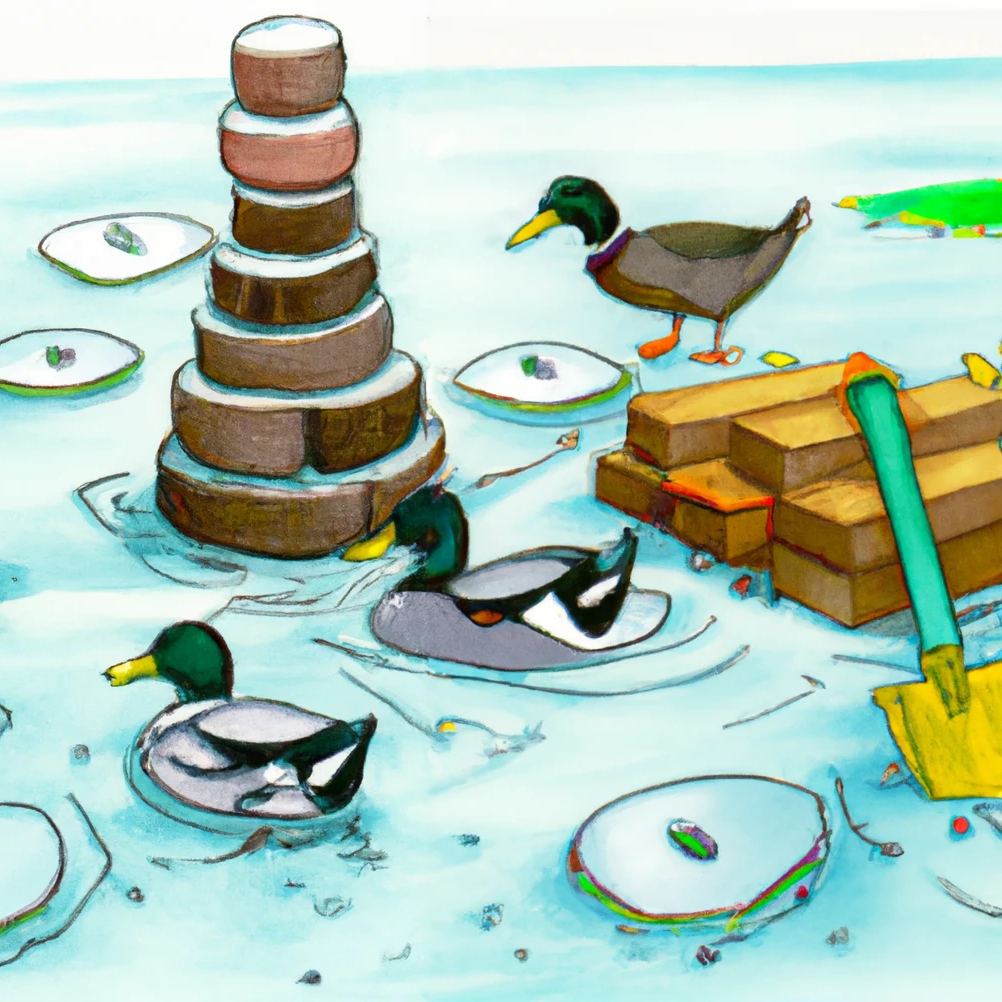
\includegraphics[width=.3\textwidth, right]{img/constructing.png}
        \captionsetup{textformat=empty,labelformat=blank}
        \caption{Generated with Dall-E. \url{https://labs.openai.com/}. ``more ducks building and working on  a high stack in the water using an excavator and tools and machines''}
\end{figure}

\epigraph{\itshape The best way to explain it is to do it.}{Lewis Caroll, \textit{Alice in Wonderland}}

We are going to present a polynomial-time preprocessing procedure giving a linear kernel for \psdom parametrized by solution size. Based on the technique first introduced by Alber et al. (\cite{Alber2004}) in 2004, an abundance of similar results to other domination problems emerged which gave us the belief we can transfer these results to \sdom. \cref{tbl:kernels} gives an overview of the status of kernels for the planar case on various domination problems. All of these results introduce reduction rules bounding the number of vertices inside so-called ``regions'' which can be obtained by a special decomposition of the planar graph. 
% TODO: Add the running time of this algorithm there.
\begin{table}[h]
\begin{minipage}[th]{\linewidth}
\setcounter{mpfootnote}{\value{footnote}}
\renewcommand{\thempfootnote}{\arabic{mpfootnote}}

\begin{tabularx}{\textwidth}{lcX}
\textbf{Problem} & \textbf{Best Known Kernel} & \textbf{Source} \\
\pdom &  $67k$ & \cite{Diekert2005}\footnotemark\\
\ptdom &  $410k$ & \cite{Garnero2018}\footnotemark \\
\psdom & $\kernelsize k$ & \textbf{This work} \\
& & \\
\peddom & $14k$  & \cite[Th. 2]{Guo2007} \\
\pefdom &  $84k$ & \cite[Th. 4]{Guo2007} \\
\prbdom &  $43k$ & \cite{Garnero2017} \\
\pcdom & $130k$  & \cite{Luo2013} \\
\pdirdom & Linear  & \cite{Alber2006}  \\
\end{tabularx}

\footnotetext[1]{There is also a master's thesis claiming a bound of 43k \cite{Halseth2016}, but a conference or journal version was not found.}
\footnotetext[2]{Improved their own results from first $694k$ \cite[Revision 2012]{Garnero2018}}
\setcounter{footnote}{\value{mpfootnote}}
\end{minipage}
\caption{An overview about existing kernels for planar dominating set variants}
\label{tbl:kernels}
\end{table}

In the following years, this approach bore fruits in other planar problems as well like 
\name{Connected Vertex Cover}\xspace ($11/3k$ in \cite{Kowalik2013}),
\name{Maximum Triangle Packing}\xspace ($624k$ in \cite{Wang2011})
\name{Induced Matching}\xspace ($40k$ in \cite{Kanj2011})
\name{Full-Degree Spanning Tree}\xspace (\cite{Guo2006})
\name{Feedback Vertex Set}\xspace ($13k$ in \cite{Bonamy2016}) and 
\name{Cycle Packing}\xspace (\cite{Garnero2019})

% TODO Where from?
In the impending years, many results generalized this approach to larger graph classes. Fomin and Thilikos started by proofing that the initial reduction rules given by Alber et al. \cite{Alber2004} can also be used to obtain a linear kernel on graphs with bounded genus $g$ (\cite{Fomin2004}).
Gutner advanced in 2008 by giving a linear kernel on $K_{3,h}$-topological-minor-free graph classes and a polynomial kernel for $K_h$-topological-minor-free graph classes (\cite{Gutner2009}). 
% TODO following required?
% In 2007 they extended it to show that graphs of bounded degeneracy are FPT (\cite{Alon2007}). 
In 2012 Philip, Raman and Sikdar showed that $K_{i,j}$-free graph classes admit a polynomial kernel for \dom (\cite{Philip2012}). 
In an attempt to extend these ideas to other problems as well, Bodlaender et al. proved that all problems expressible in counting monadic second-order logic satisfying a coverability property admit a polynomial kernel on graphs of bounded genus g (\cite{Bodlaender2016}).

These meta-results are interesting from a theoretical point of view, but the constants for the kernels obtained by these methods are too large to be of practical interest. The question of how an efficient kernel can be constructed remains. We will transfer the kernel described by Garnero and Sau in their original version of \cite[Revision 2014]{Garnero2018} for \ptdom can also be ``recycled'' for \psdom giving us an explicitly constructed kernel with ``reasonable'' small constants.

 \paragraph{The Main Idea} A given a plane graph \G with a given vertex set $D \subseteq V$ can be decomposed into at most $3 \cdot \abs{D} -6$ so-called ``regions'' (see \cref{def:region}). If $D$ is a given \sdom~of size $\abs{D}$, the total number of regions in this decomposition depends \underline{linearly} on the size of $D$. If we define \textit{reduction rules} (\cref{rgl:rone,rgl:rtwo,rgl:rthree})  minimizing the number of vertices in and around a region, we can bound the size of a reduced graph. In our case, we give rules to reduce a region down to a constant number of vertices. We can create an equivalent instance of $G$ whose number of remaining vertices lies linearly in the size of an enquiried solution. Such a reduction gives a \textit{Kernel} for \psdom.


Interestingly, the reduction rules do not rely on the decomposition itself, but rather consider the neighborhood of every pair of vertices in the graph. The decomposition itself has just used a tool for analyzing the kernel size after the reduction.

\section{Definitions}

Before giving the exact reduction rules, we need some definitions which expose some nice properties we are going to exploit. They are inspired by those given by Garnero and Sau (\ptdom in \cite[Revision 2014]{Garnero2018} or \prbdom in \cite{Garnero2017}) and reused ideas introduced by Alber et al. in \cite{Alber2004} for \pdom.

The idea is to split up the neighborhood of a single vertex and a pair of vertices into three distinct subsets which intuitively give us a level of ``confinement'' of these vertices and how closely they are related to the rest of the graph (\cite[p. 6]{Garnero2018}). 

\begin{definition}
    \label{def:nv}
    Let \G be a graph and let $v \in V$. We denote by $N(v) = \{u \in V : \{u,v\} \in E \}$ the neighborhood of $v$. We split $N(v)$ into three subsets:
    \begin{align}
        N_1(v) & = \{u \in N(v) : N(u) \setminus N[v] \neq \emptyset \}              \\
        N_2(v) & = \{u \in N(v)\setminus N_1(v) : N(u) \cap N_1(v) \neq \emptyset \} \\
        N_3(v) & = N(v) \setminus (N_1(v) \cup N_2(v))
    \end{align}
    To enhance future readability, for $i,j \in [1,3]$, we denote $N_{i,j} (v) := N_i(v) \cup N_j(v)$. Furthermore, we call a vertex $v'$ \textit{confined} by a vertex $v$, if $N(v') \subseteq N[v]$
\end{definition}

\begin{figure}[!ht]
    \label{fig:neighborhoodSingle}
    \begin{equation*}
        \tikzfig{fig/tikz/neighborhoods-single-vertex}
    \end{equation*}
    \caption[The neighbordhood of a single Vertex $v$]{\textit{The neighborhood of a single vertex v split to $N_1(v)$ (purple), $N_2(v)$ (blue), and $N_3(v)$ (green). $N_1(v)$'s are those having neighbors outside $N(v)$, $N_2(v)$'s are a buffer between $N_1(v)$ and $N_3(v)$, and $N_3(v)$-vertices are confined in $N(v)$}.}
\end{figure}

\begin{xltabular}{\textwidth}{lX}
\textbf{$\mathbf{N_1(v)}$} & is all the neighbors of $v$ which have at least one adjacent vertex that is outside of $N(v)$ and therefore connects $v$ with the rest of the graph. They can belong to a \sdom. \\

\textbf{$\mathbf{N_2(v)}$} & is all neighbors of $v$ that have at least one neighbor in $N_1(v)$. These vertices do not have any function as a dominating vertex and can be seen as a \textit{buffer} bridging $N_1(v)$-vertices with those from $N_3(v) \cup \{ v \}$. Furthermore, they are useless as witnesses, because either we can replace them with $v$ (sharing the same neighborhood) or when being a witness for $v$, we replace it with a $z \in N_1(v)$. \\

$\mathbf{N_3(v)}$ & vertices are sealed off from the rest of the graph. They are useless as dominating vertices: For all $z \in N_3(v)$ it holds that  $N(z) \subseteq N(v)$ by definition and thus, we would always prefer $v$ as a dominating vertex instead of $z$. Nevertheless, they can be important as a witness for $v$ in the case where it is the only neighbor of $v$ (this $N_1(v) \cup N_2(v) =\emptyset$). We are using this observation in \cref{rgl:rone} where we shrink $\abs{N_3(v)} \leq 1$.
\end{xltabular}

% TODO What can they dominate
% TODO This sentence? Every path to a vertex outside N(v) will take more than 2 steps. 
% TODO Grammar 

Next, we are going to extend this notation to a pair of vertices. Using this, \cref{rgl:rtwo} will later try to reduce the neighborhood of two vertices, and similar to \cref{def:nv}, we observe nice properties. Again, the idea is to classify how strongly the shared neighborhood of two vertices $N(v) \cup N(w)$ is connected to the rest of the graph.

%TODO Where is it used?
\begin{definition}
    Let \G be a graph and $v,w \in V$. We denote by $N(v,w) := N(v) \cup N(w)$ the shared neighborhood of the pair $v,w$ and split $N(v,w)$ into three distinct subsets:
    \begin{align}
        N_1(v,w) & = \{u \in N(v,w) \mid N(u) \setminus (N(v,w)\cup \{v,w\}) \neq \emptyset \}  \\
        N_2(v,w) & = \{u \in N(v,w)\setminus N_1(v,w) \mid N(u) \cap N_1(v,w) \neq \emptyset \} \\
        N_3(v,w) & =  N(v,w) \setminus (N_1(v,w) \cup N_2(v,w))
    \end{align}
    Again, for $i,j \in [1,3]$, we denote $N_{i,j}(v,w) = N_i(v,w) \cup N_j(v,w)$.
\end{definition}

\textbf{$N_1(v,w)$} contains those vertices connected with the rest of the graph by at least one vertex not in the neighborhood of $v$ or $w$, \textbf{$N_2(v, w)$}-vertices are a \textit{buffer} between those from $N_3(v,w) \cup \{v, w\}$ and $N_1(v,w)$, and \textbf{$N_3(v,w)$} contains vertices isolated from the rest of the graph. You can see an example in \cref{fig:neighborhoodDouble}. 

\begin{figure}[!ht]
    \begin{equation*}
        \tikzfig{fig/tikz/neighborhoods-two-vertices}
    \end{equation*}
    \caption[$N_i(v,w)$]{\textit{The neighborhood of a pair of vertices. Vertices from $N_3(v,w)$ are colored green, $N_2(v,w)$'s blue and $N_1(v,w)$'s purple.
    NOte that $z \in N_1(w)$, because there is an edge to a neighbor of $v$, but $z \notin N_1(v,w)$ (and rather $z \in N_3(v,w)$)}.}
    \label{fig:neighborhoodDouble}
\end{figure}


A vertex $v \in N_i(v)$ is not necessarily also in $N_i(v,w)$! Observe the vertex $z$ in \cref{fig:neighborhoodDouble}. Unlike $N_i(v)$ in every $N_i(v,w)$ ($i \in [3]$) can be in an optimal \sdom (compare \cref{fig:alldominating} for an example in each of the sets).

\begin{figure}[!ht]
    \begin{equation*}
        \tikzfig{fig/tikz/ntwoimportant}
    \end{equation*}
    \caption[$N_i(v,w)$]{\textit{Left:} $\{d_1, d_2\}$ with $d_2 \in N_2(v,w)$ form the only minimal \sdom. \textit{Right:} $d_1 \in N_1(v,w)$ and $d_2 \in N_3(v,w)$ optimal.}
    \label{fig:alldominating}
\end{figure}


%\begin{figure}[ht]
%    \begin{equation*}
%        \tikzfig{fig/tikz/neighborhoods-odd}
%    \end{equation*}
%    \caption[Counterexample]{\textit{The vertex $z$ is in $N_1(v)$, because there is an edge pointing outside of $N(v)$ to $w$. Contrary, it is not in $N_1(v,w)$, but now  belongs to $N_3(v,w)$, because we are considering the ``shared'' neighborhood}}
%    \label{fig:neighborhoodWeird}
%\end{figure}

\subsection{Reduced Graph}

Before stating the reduction rules, we want to clarify when we consider a graph to be a \textit{reduced}. 

\begin{definition}[Reduced Graph {\cite[p. 13]{Garnero2018}} and \cite{Garnero2017}]\label{def:reduced}
    A Graph G is reduced under a set of rules if either none of them can be applied to G or the application of any of them creates a graph isomorphic to G.
\end{definition}

This definition differs from the definition usually given in literature where a graph G is \textit{reduced} under a set of reduction rules if none of them can be applied to G anymore (compare e.g. \cite{Fomin2019}). Some of our reduction rules (\cref{rgl:rone} or \cref{rgl:rtwo}) could be applied \textit{ad infinitum} creating an endless loop that does not change G any more. Our definition guarantees termination in that case. All of the given reduction rules are local and only need the neighborhood of at most two vertices and replace them partially with gadgets of constant size. Now checking whether a graph after applying the rule has been isomorphically changed can be trivially accomplished in constant time.

In our case, we say G is reduced if all of the \cref{rgl:rone,rgl:rtwo,rgl:rthree} have exhaustively been applied.

\subsection{Regions in Planar Graphs}

Alber et al. gave in \cite{Alber2004} a novel approach to look at planar graphs. In their analysis, they stated a constructive algorithm that decomposes a planar graph into local ``regions''. Vaguely said, a region is a set of vertices that are enclosed by a boundary path in a fixed planar embedding of the graph.

The following definitions are based on those given by Garnero and Sau in \cite[Revision 2014]{Garnero2018} and will lead toward a clean definition of a \textit{region} and what we understand as a \dreg. More detailed explanations and concrete examples can be found in their paper.

\begin{definition}
    Two simple paths $p_1, p_2$ in a plane graph G are \underline{confluent} if:
    
    \begin{enumerate}
        \item they are vertex-disjoint
        \item they are edge-disjoint and for every common vertex $u$, if $v_i, w_i$ are the neighbors of $u$ in $p_i$, for $i \in [1,2]$, it holds that $[v_1, w_1, v_2, w_2]$, or
        \item they are confluent after contracting common edges
    \end{enumerate}
\end{definition}

% TODO MORE TEXT HERE

\begin{definition}
    Let \G be a plane graph and let $v,w \in V$ be two distinct vertices. A \underline{ region $R(v,w)$} (synonymy denoted as  $vw$-region) is a closed subset of the plane, such that:
    \begin{enumerate}
        \item the boundary of R is formed by two confluent simple $vw$-paths with length at most 3
        \item every vertex in R belongs to $N(v,w)$, and
        \item the complement of R in the plane is connected.
    \end{enumerate}
    
    We denote with $\partial R$ the boundary of $R$ and by $V(R)$ the set of vertices laying (on the plane embedding) in $R$. Furthermore, we call $\abs{V(R)}$ the \textit{size of the region}.
    
    The poles of R are the vertices $v$ and $w$. The boundary paths are the two $vw$-paths that form $\partial R$
    
\end{definition}

\begin{definition}
    Two regions $R_1$ and $R_2$ are non-crossing, if:
    \begin{enumerate}
        \item $(R_1 \setminus \partial R_1) \cap R_2 = (R_2 \setminus \partial R_2) = \emptyset$, and
        \item the boundary paths of $R_1$ are pairwise confluent with the ones in $R_2$
    \end{enumerate}
\end{definition}

We now have all the definitions ready to formally a maximal \dreg on planar graphs:

\begin{definition}\label{def:region}
    Given a plane graph \G and $D\subseteq V$, a \underline{$D-region$ Decomposition} of G is a set $\mathfrak{R}$ of regions with poles in D such that: 
    \begin{enumerate}
        \item for any $vw$-region $R \in \mathfrak{R} $, it holds that $D \cap V(R) = \{v, w\}$, and
        \item all regions are pairwise non-crossing.
    \end{enumerate}
    We denote $V(\mathfrak{R}) = \bigcup\limits_{R \in \mathfrak{R}} V(R)$. 
    
    \noindent A \dreg is \underline{maximal} if there is no region $R \notin \mathfrak{R}$ such that $\mathfrak{R}' = \mathfrak{R} \cup \{R\}$ is a \dreg~with $V(\mathfrak{R}) \subsetneq V(\mathfrak{R}')$.
\end{definition}


\cref{fig:maxRegionDecompose} gives an example of how to decompose a graph into a maximal $D-region$ decomposition with a given \sdom $D$ of size 3.

\begin{figure}[!ht]
    \begin{equation*}
        \tikzfig{fig/tikz/region-example}
    \end{equation*}
    \caption[Region Decomposition]{\textit{Left: A maximal \dreg $\mathfrak{R}$, where $D = \{d_1,d_2,d_3\}$ form a \sdom. There are two regions between $d_2$ and $d_1$ (purple and pink), one region between $d_1$ and $d_3$ (green) and one region between $d_2$ and $d_3$ (purple). Observe that some neighbors of $d_1$ are not part of any $vw$-region. Our reduction rules are going to take care of them and bound these number of vertices to obtain the kernel. Right: The corresponding underlying multigraph $G_{\mathfrak{R}}$. Every edge denotes a region between $d_i$ and $d_j$}}\label{fig:maxRegionDecompose}
\end{figure}

% TODO: Wording: "kernel" is precise enough here.
We are introducing a special subset of a region, namely \textit{simple region} where every vertex is a common neighbor of $v$ and $w$. They will appear in many unexpected astonishing places and are an important tool to operate on small parts of a plane graph. The upcoming \cref{rgl:rthree} will bound the size of these \textit{simple regions}. Interestingly, in the first version of the paper about the linear kernel for \ptdom (\cite[Revision 2014]{Garnero2018}), they were not given independently but covered by one of their reduction rules (Rule 2). As it turned out, the analysis is getting simpler if we treat them in a separate rule (In our case: \cref{rgl:rthree}) and so did Garnero and Sau in a revised version of their paper four years later (\cite{Garnero2018}).

\begin{minipage}{\textwidth}
\begin{definition}
    A simple $vw$-region is a $vw$-region such that:
    \begin{enumerate}
        \item its boundary paths have length at most 2, and
        \item $V(R) \setminus \{v,w\} \subseteq N(v) \cap N(w)$.
    \end{enumerate}

\end{definition}
\end{minipage}

\cref{fig:simpleRegionExample} shows an example of a simple region containing 9 distinct vertices.

\begin{figure}[!ht]
    \begin{equation*}
        \tikzfig{fig/tikz/simple-region-example}
    \end{equation*}
   \caption[A Simple Region]{\textit{A simple region with two vertices from $N_1(v,w)$ (purple) setting the boundary, two vertices from $N_2(v,w)$ (blue) and some vertices from $N_3(v,w)$ (green) in between.}}
    \label{fig:simpleRegionExample}
\end{figure}

In the analysis, we will also use properties of the \textit{underlying multigraph} of a \dreg $\mathfrak{R}$. Refer to \cref{fig:maxRegionDecompose} for an example.

\begin{minipage}{\textwidth}
\begin{definition}\label{def:unterlyingMG}
    Let \G be a plane graph, let $D \subseteq V$ and let $\mathfrak{R}$ be a \dreg of G. The underlying multigraph $G_\mathfrak{R} = (V_\mathfrak{R}, E _\mathfrak{R})$ of $\mathfrak{R}$ is such that  $V_\mathfrak{R} = D$ and there is an edge $\{v,w\} \in E_\mathfrak{R}$ for each vw-region $R(v,w) \in \mathfrak{R}$
\end{definition}
\end{minipage}

\section{The Big Picture}
\cref{fig:overview} gives a high-level view of how we are going to obtain the linear kernel for \psdom. We will first derive three different reduction rules (\cref{rgl:rone,rgl:rtwo,rgl:rthree} are green in the overview), prove that they preserve the solution size $k$ and run in polynomial-time. 
Then we use the existence of a maximal \dreg~$\mathfrak{R}$ on planar graphs to bound the number of vertices that fly around a given region $R \in \mathfrak{R}$. This will lead us towards a bound on the number of vertices inside R. Furthermore, we observe that the number of vertices that are not enclosed in R, but lie outside the border is bounded, too. We will often encounter hidden simple regions which are reduced by \cref{rgl:rthree} and therefore of constant size by \cref{lemma:simpleregionbound}. As we know that the total number of regions R in the \dreg is linear in $k$, we obtained a linear kernel for the \psdom as well.
\begin{figure}[!ht]
    \begin{equation*}
    \scalebox{.9}
    {
        \tikzfig{fig/tikz/overview}
    }
    \end{equation*}
    \caption[Structure of the Proof]{\textit{The plan for obtaining a linear kernel for \psdom. Starting with the reduction rules (Green) we will derive the number of vertices inside and outside of a $vw$-region.}}\label{fig:overview}
\end{figure}

\section{The Reduction Rules}

Following the ideas proposed by Garnero and Sau in \cite[Revision 2014]{Garnero2018}, we state reduction rules that after exhaustive application will expose a linear kernel. We note that especially for \cref{rgl:rtwo}, we relied on the first revision of the paper because in the following years their kernel size was improved for the cost of making them more specific to \ptdom and we saw that the latest rules stated will not work for \psdom. 
The main challenge in all of those rules is to maintain the witness properties of the graph because a vertex inside a region can be important as a witness for vertices in another region and can not always simply be reduced. Therefore a more sophisticated analysis is required. 
\subsection{Reduction Rule I: Getting Rid of unneccessary  $N_3(v)$ vertices}

% Maybe we can even remove all N_3's because later, only the case v in a pair could be important. We do not have a connected graph.

The idea of the first rule is the observation that a vertex $v' \in N_{2,3}(v)$ dominates $v$ and possibly vertices from $N_2(v)$ and $N_3(v)$. As $N(v') \subseteq N(v)$ and the \cref{fact:witnessTwin} that a witness for $v'$ is also witness for $v$, we can use $v$ instead of $v'$ as a dominating vertex. Therefore, we can remove $N_{2,3}$ from the graph. Nevertheless, $v'$ can be a witness for $v$ itself and might be required in a solution. Our rule ensures that at least one $N_3(v)$-vertex is preserved. An example for this rule is shown in \cref{fig:ruleOne}.

\begin{fact}\label{fact:witnessTwin}
Let \G, $v \in V$ and $v' \in N_{2,3}(v)$. Any witness $w \neq v$ for $v'$ is also a witness for $v$. % Reformulate as v can be a witness for $w'$
\end{fact}
\begin{proof}

By assumption $v'$ is witnessed by a vertex $w \neq v$ with $d(v', w) \leq 2$. It follows directly from the definition of $v' \in N_{2,3}(v)$ that $N(v') \subseteq N[v]$ and hence $v'$ is \textit{confined} inside the neighborhood of $v$. Every path $P = (v', n, w)$ from $v'$ to possible witness $w$ within two steps must pass at least one vertex $n \in N[v]$ as all neighbors. This implies that there exists also a path from $v$ to $w$ with a length of at most two and $v$  

% Maybe add a note that it can also point outside of N(v)
% we know that $w$ is either $v$, a direct neighbor of $v$ or can be reached via one step over a $N_1(v)$ vertex, hence $w \in N(v) \cup \bigcup\limits_{z \in N_1(v)} N(z) $. Clearly, $d(v, w) \leq 2$.
\end{proof}



\begin{figure}[!ht]
    \begin{equation*}
        \tikzfig{fig/tikz/ruleOne}
    \end{equation*}
    \caption{\textit{Simplifying $N_{23}(v)$: As $N_3(v) \geq 1$, we remove $N_{23}(v)$ and add a new witness $v'$. $N_1(v)$ remains untouched.}}
    \label{fig:ruleOne}
\end{figure}

\begin{rgl}\label{rgl:rone}
    Let \G be a graph and let $v \in V$. If $\abs{\Nthreev} \geq 1$:
    \begin{itemize}
        \item remove $N_{2,3}(v)$ from G,
        \item add a vertex $v'$ and an edge $\{v, v'\}$
    \end{itemize}
\end{rgl}

\noindent We can now prove the correctness of this rule.

\begin{lemma}\label{lemma:correctnessone}
    Let \G be a graph and let $v \in V$. If $G'$ is the graph obtained by applying \cref{rgl:rone}   on $G$, then G has a \sdom of size k if and only if G' has a \sdom of size k.
\end{lemma}
\begin{proof}
    \begin{enumerate}
        \item[$\Rightarrow$] Let $D$ be a \sdom in $G$ of size k. 
        Because \cref{rgl:rone} has been applied, we can assume $N_{2,3}(v) \neq \emptyset$ in $G$. 
        
        To dominate all vertices from $N_3(v)$ we either need $v \in D$ or at least one other vertex $d \in N_{2,3}(v) \cap D$. In the latter case, we can replace this vertex by $v$ directly. By \cref{fact:witnessTwin}, we know that a witness for $d$  (which is not  $v$) is also a witness for $v$ and therefore, the replacing preserves the \sdom. Henceforth, we assume $v \in D$ and $N_{2,3}(v)$ is already dominated by $v$.

        If \cref{rgl:rone} has removed at least one dominating vertex from $N_{2,3}(v)$, we set $D' = D \setminus N_{2,3}(v) \cup \{v'\}$ otherwise $D = D'$. 
        In the first case this vertex in $N_{2,3}(v) \cap D$ could have possible been a witness for $v$, so we select $v' \in D'$ as a witness for $v$ ensuring $D'$ to be a \sdom. In both cases $v'$ is by assumption dominated by $v$ and  $\abs{D} \leq \abs{D'}$.

        \item[$\Leftarrow$]  Assume $D'$ to be a \sdom in $G'$. We can assume that $v \in D'$, because $v'$ has to be dominated and it is always better to choose $v$ instead of $v$.

        If $v' \in D'$ is a witness for $v$ in $G'$, we have to preserve a witness in $G$ as well. As we know that $N_3(v) \neq \emptyset$, we can replace it by an arbitrary vertex $d \in N_3(v)$ in $G$. 
        
        In the second case, the witness for $v$ came either from a vertex $o \in N_1(v)$ or some neighbor $N(o) \setminus N(v)$ outside the neighborhood of $v$ which has not been touched by this reduction rule. 
        In summary, if $v' \in D'$, we set $D = D' \cup \{d\} \setminus \{v'\}$ for any $d \in N_3(v)$ and otherwise $D = D'$. In both cases, $N_{2,3}(v)$ is dominated by $v$ and $\abs{D} = \abs{D'}$.
    \end{enumerate}
\end{proof}

\begin{lemma}
    A plane graph $G$ of $n$ vertices is reduced under \cref{rgl:rone} in time $\mathcal{O}(n)$
\end{lemma}
\begin{proof}
    As \cref{rgl:rone} stayed the same, the proof directly follows \cite[Lemma 2]{Alber2004}.
\end{proof}

Note that we need our definition of a reduced instance given in \ref{def:reduced}. If \cref{rgl:rthree} is being applied, it will still leave us with a vertex $z\in N_3(v)$ allowing this rule to be applied again.

\subsection{Reduction Rule II: Shrinking the Size of a Region}

The second rule is the heart of the whole reduction and it aims to minimize the neighborhood of two distinct vertices. The rule follows Garnero and Sau's approach in one of the early versions of \cite[Revision 2014]{Garnero2018} for \ptdom. The reduction rules given in the latest version (\cite[Revision 2018]{Garnero2018}) were not directly transferable to \psdom, because they heavily rely on the property of a \tdom that a witness $w$ for $v$ \textbf{must} be a direct neighbor of $w$. In the case of the more relaxed \sdom, the witness is allowed to have more range.

% TODO: Force connectivity, improve kerne bound
% TODO: Reformulate
% Extending the approach for a linear kernel for \dom proposed by Alber et al. in \cite{Alber2004}, Garnero and Sau transferred these results in \cite{Garnero2018} to the \tdom problem. 

It can be observed that in the worst case four vertices are needed to semi-totally dominate $N(v,w)$ of two vertices $v,w \in V$: $v$, $w$ and two witnesses for them. Exemplary, observe the graph consisting of two distinct $K_{1,m}$ with $m \in \mathbb{N}$ with centers $v$ and $w$.

Before we give the concrete reduction rule, we need to define three sets. Intuitively, we first try to find a set $\tilde D \subseteq N_{2,3}(v,w)$ of size at most three dominating $N_3(v,w)$ without using $v$ or $w$. If no such set exists, we allow $v$ (resp. $w$) and try to find one again. If we now find such a set, we can conclude that $v$ ($w$) must be part of a solution.

\begin{definition}
Let \G be a graph and let $v,w \in V$. We now consider all the sets that can dominate $N_3(v,w)$:
\begin{align}
    \Dvw & = \{ \tilde D \subseteq N_{2,3}(v,w)            \mid N_3(v,w) \subseteq \bigcup_{v \in \tilde D} N(v),\ |\tilde D| \leq 3                  \} \\
    \Dv  & = \{ \tilde D \subseteq N_{2,3}(v,w) \cup \{v\} \mid N_3(v,w) \subseteq \bigcup_{v \in \tilde D} N(v),\ |\tilde D| \leq 3,\ v \in \tilde D \} \\
    \Dw  & = \{ \tilde D \subseteq N_{2,3}(v,w) \cup \{w\} \mid N_3(v,w) \subseteq \bigcup_{v \in \tilde D} N(v),\ |\tilde D| \leq 3,\ w \in \tilde D \}
\end{align}

Furthermore, we shortly denote $\bigcup \Dv = \bigcup\limits_{D \in \Dv}D $ and $\bigcup \Dw = \bigcup\limits_{D \in \Dw}D$.
\end{definition}

Assuming that $v$ and $w$ are closely connected with $d(v,w) \leq 2$, it might suffice to consider only sets of size at most three, because an intermediate vertex could witness $v$ and $w$ at the same time. In the later analysis, the \dreg exactly creates regions around $N(v,w)$ requiring at least one path from $v$ to $w$ lengthed two. As the following rule is only used to locally investigate such regions, we could add the requirement of a distance of two to it and work with sets of size at most three. We believe that this could further improve the kernel. 

We are now ready to state \cref{rgl:rtwo}:

\begin{rgl}\label{rgl:rtwo}
    Let \G be a graph and $v,$ be two distinct vertices from $V$. If $\mathbf{\Dvw = \emptyset}$ we apply the following:
    \begin{caseof}
        \case{if $\Dv =  \emptyset$ and $D_w = \emptyset$\label{case:c1}}

        \vspace{-5mm}
        \begin{itemize}
            \item Remove $N_{2,3}(v,w)$
            \item Add vertices $v'$ and $w'$ and two edges $\{v, v'\}$ and $\{w, w'\}$
            \item If there was a common neighbor of $v$ and $w$ in $N_{2,3}(v,w)$, add another vertex $y$ and two connecting edges  $\{v, y\}$ and $\{y, w\}$
            \item If there was no common neighbor of $v$ and $w$ in $N_{2,3}(v,w)$, but at least one path of length three from $v$ to $w$ via only vertices from $N_{2,3}(v,w)$, add two vertices $y$ and $y'$ and connecting edges $\{v,y\}$, $\{y, y'\}$ and $\{y', w\}$
        \end{itemize}
        \case{if $\Dv \neq  \emptyset$ and $D_w = \emptyset$\label{case:c2}}

        \vspace{-5mm}
        \begin{itemize}
            \item Remove $N_{2,3}(v)$
            \item Add $\{v, v'\}$
        \end{itemize}
        
        \case{if $\Dv =  \emptyset$ and $D_w \neq \emptyset$\label{case:c3}} This case is symmetrical to \cref{case:c2}.
    \end{caseof}
\end{rgl}

%% Description Case 1
In \cref{case:c1}, we know by \cref{fact:f2} that $v$ and $w$ must be in $D$. Therefore, we introduce two forcing vertices $v'$ and $w'$ in $G'$ and remove $N_{2,3}(v,w)$ as these vertices are dominated by $v$ and $w$.
But if we remove $N_{2,3}(v,w)$ entirely, we could lose solutions: First, the case that $v$ is a direct witness of $w$ ($d(v,w) = 2$) and that there is one intermediate witness on a path of length three from $v$ to $w$ via vertices in $N_{2,3}(v,w)$, which could be a witness for both $v$ and $w$ at the same time. 

Note that if we would not distinguish between these two cases and had added one intermediate vertex in both of them, we would possibly have generated some wrong solutions, because $v$ could always witness $w$.


Again by \cref{fact:f2} we know for \cref{case:c2,case:c3} that $v \in D$ and similar to \cref{rgl:rone} we can simplify the neighborhood $N_{2,3}(v)$. \cref{fact:f1} states, that these vertices are only useful for witnessing $v$, but do not go beyond what $v$ already witnesses. Observe that removing $N_{2,3}$ can not break any connectivity as all vertices in  $N_{2,3}(v)$ are confined in $v$. The cases where $\Dv \neq \emptyset$ and $\Dw \neq \emptyset$ are not required and in a later analysis only the existence of these two sets is required and the application of \cref{rgl:rthree} will be critical.

Before proofing \cref{rgl:rtwo} we will deduce some \textit{facts} which are implied by the definitions above. These facts justify the definition of the sets $\Dvw$, $\Dv$ and $\Dw$.

\begin{fact}\label{fact:f1}
    Let \G be a graph, let $v,w \in V$, and let $G'$ be the graph obtained by the application of \cref{rgl:rtwo} on $v,w$. If $\Dvw = \emptyset$, then G has a solution if and only if it has a solution containing at least one of the two vertices $\{v,w \}$.
\end{fact}
\begin{proof}
Because $\Dvw = \emptyset$, any SDS of $G$ has to contain $v$ or $w$, or at least four vertices from $N_{2,3}(v,w)$. In the second case, these four vertices can be replaced with $v$, $w$ and two neighbors of $v$ and $w$ still forming a \sdom.
\end{proof}

The second fact states that if  $\Dv$ (resp. $\Dw$) is empty, too, we only need to consider solutions containing $w$ (or $v$):

\begin{fact}\label{fact:f2}
    Let \G be a graph, let $v,w \in V$, and let $G'$ be the graph obtained by the application of \cref{rgl:rtwo} on $v, w$. If $\Dvw = \emptyset$ and $\Dw = \emptyset$ (resp. $\Dv = \emptyset$) then $G'$ has a solution if and only if it has a solution containing $v$ (resp. $w$).
\end{fact}
\begin{proof}
As $\Dv = \emptyset$, no set of the form $\{v\}$, $\{v, u\}$ or $\{v, u, u'\}$ with $u, u' \in N_{2,3}(v,w)$ can dominate $N_3(v,w)$. Since also $\Dvw = \emptyset$ any SDS of G has to contain $v$ or at least four vertices by \cref{fact:f1}. In the last case, we again replace these four vertices with $v$, $w$ and two neighbors respectively and we can conclude that $v$ belongs to the solution.
\end{proof}

% On the opposite side, if $\Dvw \neq \emptyset$, we have ... 

\noindent Now we are ready to prove the correctness of \cref{rgl:rtwo}
\begin{lemma}\label{lemma:correctnesstwo}
    Let \G be a plane graph, $v, w \in V$ and \GB be the graph obtained after application of \cref{rgl:rtwo} on the pair $\{v, w\}$. Then G has \sdom of size k if and only if G' has \sdom of size k.
\end{lemma}
\begin{proof}
    We will prove the claim by analyzing the different cases of the rule independently.     
    \begin{enumerate}
        \item[$\Rightarrow$] Consider a \sdom $D$ in $G$. We show that $G'$ also has a SDS with $\abs{D'} \leq \abs{D}$. By assumption, we have $\Dvw = \emptyset$.
        \begin{enumerate}
            \item  $ \Dv = \emptyset  \wedge \Dw = \emptyset $: By applying \cref{fact:f2} twice, we know that both  $v, w \in D$. Therefore, $v'$,$w'$, and potentially $y$ and $y'$ are dominated by $v$ or $w$ in $G'$.
            
            We now have three cases: Either $v$ and $w$ have their own witnesses (e.g. via two distinct $N_1(v,w)$-vertices); they are of distance three and share one witness on a path from $v$ to $w$ (which could go through $N_{2,3}(v,w)$ and therefore will be kept by the vertices $y$ and $y$) is required, or they can be of distance less than three, such that they already witness each other directly. 
            Furthermore, a direct edge $\{v,w\}$ will not be reduced. 

            We will now build $D'$ depending on which vertices from $D \cap N_{2,3}(v,w)$ have been removed. 
            % Add figure.
            \begin{itemize}
                \item If the rule has not removed any $d \in D$, we simply set $D' = D$. If $v$ was a witness for $w$ (and vice versa), \cref{rgl:rtwo} will preserve it by introducing the vertex $y$. Otherwise, these witnesses are preserved.
                \item If $d(v,w) > 3$, then $v$ and $w$ are not sharing any common witnesses. 
                If the rule has removed a vertex from $D \cap N(v)$, we set $D' = D \setminus N_{2,3}(v,w) \cup \{v'\}$.
                If the rule has removed a vertex from $D \cap N(w)$, we  set $D' = D \setminus N_{2,3}(v,w) \cup \{w'\}$.
                If the rule has removed a vertex from $(D \cap N(v))$ and a vertex from $(D \cap N(w))$, we set $D' = D \setminus N_{2,3}(v,w) \cup \{v', w'\}$.
                \item If $d(v,w) = 3$ and the vertices $y$ and $y'$ get introduced preserving one path from $v$ to $w$, because there have been a path via $N_{2,3}(v,w)$-vertices containing a single witness for both $v$ and $w$.
                If the rule removed a dominating vertex $D \cap N_{2,3}(v, w)$, we set $D' = D \setminus N_{2,3}(v,w) \cup \{y\}$. Note that we could also choose $y' \in D'$, because $y$'s only function is to be a single witness for $v$ and $w$ and every other vertex it could be a witness for, will also be witnessed by $v,w \in D'$ (\cref{fact:f1}).
                \item If $d(v,w) \leq 2$, then $v$ and $w$ directly witness each other and the reduction must preserve this relation, which is accomplished by introducing the single bridging vertex $y$. 
                Even if the rule has removed a vertex $z \in D \cap N_{2,3}(v,w)$, we can ignore that, because \cref{fact:f1} states that $v$ and $w$ will witness the same vertices as $z$ did. Hence, we set $D' = D \setminus N_{2,3}(v,w)$.
            \end{itemize}
            
            In all of the cases, it follows that $D'$ is a SDS of $G'$ with $\abs{D'} \leq \abs{D}$ 
            
            \item  $ \Dv \neq \emptyset  \wedge \Dw = \emptyset$: As $\Dw = \emptyset$ and \cref{fact:f2}, we know that $v \in D$ and $v$ dominates $N_{2,3}(v)$. 
            If a vertex $d \in D \cap N_{2,3}(v)$ was removed, we set $D' = D \setminus N_{2,3}(v) \cup \{v'\}$, else $D' = D$.
            Deleting dominating vertices $d \in D \cap N_{2,3}(v)$ does not destroy the witness properties of the graph, because by \cref{fact:f1} we know that everything $d$ could witness, is also witnessed by $v$. 
            If $d$ was a witness for $v$, we have replaced it with $v'$ in $G'$.
            Note that otherwise a vertex from $N_1(v) \cup \{ p \in (N(z) \setminus N(v)) | z \in N_1(v) \}$ is a witness for $v$ that is not touched by this reduction. Clearly, $\abs{D'} \leq \abs{D}$ holds.
            \item  $ \Dv = \emptyset  \wedge \Dw \neq  \emptyset $: Symmetrical to previous case.
        \end{enumerate}

        \item[$\Leftarrow$] Let $D'$ be a \sdom in $G'$ and $\Dvw =  \emptyset$. We show that $G$ has a SDS $D$ with $\abs{D} \leq \abs{D'}$ by distinguishing the different cases again. 
        \begin{enumerate}
            \item  $\Dv = \emptyset \wedge \Dw = \emptyset$: In any case we know that $v,w \in D$ to dominate $v'$ and $w'$ and therefore also dominating $N_{2,3}(v,w)$ in $G$. To preserve the distance $d(v,w)$ the rule might have introduced additional vertices $y$ and $y'$.            
            \begin{itemize}
                \item If only $y$ was introduced we know that there was a common neighbor $n \in N(v) \cap N(w)$ of $v$ and $w$. $y$ allows $v$ to witness $w$ (and vice versa) and is not part of a solution itself. (assuming $y \notin D'$). Hence, we set $D = D'$.
                \item If $y$ and $y'$ were added, a solution could use one of them to provide a single witness for $v$ and $w$. There exists a path $p = (v, n_1, n_2, w)$ from $v$ to $w$ in $G$ only using vertices from $N_{2,3}(v,w)$. As $n_1$ and $n_2$ both witness $v$ and $w$, we put one of them in $D$ if at least one of $y$ or $y$ are dominating vertices in $G'$.
                Hence, if $y \in D'$ or $y \in D'$, we set $D = D' \setminus \{y,y'\} \cup \{n_1\}$.
            \end{itemize}
            \item  $\Dv \neq \emptyset \wedge \Dw = \emptyset$: Clearly, $v \in D'$ to dominate $v'$. If $v \in D'$, we set $D =  D' \setminus \{v'\} \cup d$ for some vertex $d \in N_{2,3}(v,w)$ and otherwise $D = D'$. If $v'$ was the witness of $v$, it is now replaced by $d$ and $D$ is an SDS with $\abs{D} \leq \abs{D'}$.
            \item  $\Dv = \emptyset \wedge \Dw \neq \emptyset$: Symmetrical to previous case.
        \end{enumerate} 
        In all cases, we have shown that $\abs{D} \leq \abs{D'}$ and $D$ is a \sdom of $G$.
    \end{enumerate}

\end{proof}
% What happens if D != empty?
\subsection{Reduction Rule III: Shrinking Simple Regions}

If two vertices $v$ and $w$ share enough neighbors with each other, we can sometimes conclude at least one of them to be in a solution. 

By planarity, a \textit{simple region} has at most two vertices from $N_1(v,w)$ (namely the border $\partial$), two vertices from $N_2(v,w)$ connected to the border and unlimited $N_3(v,w)$ vertices squeezed in the middle.

With a more sophisticated analysis, we were able to modify this rule such that the bound given in \cite{Garnero2018} remained valid although we might have to add some more vertices as orginally described.

%  In order to gain the same bound as .

%We notice that a reduction must preserve the $N_1(v,w)$ vertices, because they can be important as dominating vertices. 
% Unlike other regions (where we would need three vertices in the worst case), a simple region can be semitotally dominated by at most two vertices: $v$ and $w$, because $v$ instantly witnesses $w$. Therefor we asked in which cases \underline{choosing exactly one vertex in $N(v) \cap N(w) \setminus N_1(v,w)$} can expose a better solution than picking $v$ and $w$. 

% TODO Refer to 4.5 figure with simple regions

% Note a N_3(v,w) can also be on the border!
%General Idea: sharing neighbors already force v or w into ds
%
%A worst-case shared neighborhood has exactly 5 vertices (see fig.)
%
%We know that $v$ witnesses $w$ (and vice versa) and therefore, we can always semitotal dominate with at most to vertices. 
%
%Sometimes it is possible to cover all with only one vertex from $N_x$
%
%choosing two of the shared vertices yields a better solution than $v$ and $w$: One common neighbor is already enough to dominate $v$ and $w$ and can be witnesses by a  
%
%Furthermore, we also know that $v$ directly witnesses $w$ 
%
%There are some situations where a 
%
%Furthermore, in order to witness   
% PRoblem
%The lowest number of shared vertices we could come up with 
%
%
%While first directly embedding the following \cref{rgl:rthree} into \cite[Revision 2014]{Garnero2018} into \cref{rgl:rtwo}, Garnero and Sau decided in \cite[Revision 2018]{Garnero2018} to the reduction into a separate rule simplyfing the further analysis. 
%
%For a total dominating set, it is sufficient to check ...
%
%
%This reduction rule is a ``swiss-army-knife'' and simple regions found at various places will  
%
%For \tdom it is sufficient to replace these vertices with one single intermediate vertex $h$, because no solution would use $h$ without either including $v$ or $w$ as well as $h$ must also be dominated. Resembling an ``OR''-Gadget.
%
%% TODO: Refactor.
%However, for \sdom the situation is a bit different: There could be another witness for $h$ than $v$ or $w$ (for example a $N_1(v,w)$-vertex) and we might generate smaller solutions. Therefore, our gadget consists of two vertices $h_1$ and $h_2$. A solution would either contain $h_1$ and $h_2$ or at least $v$ or $w$. In the first case, we replace it with $v$ and $w$ which is still a \sdom.
%
%A vertex on the border $\partial R$ must not necessarily be in $N_1(v,w)$ if it has no neighbors outside. In that case it belongs to $N_3(v,w)$. To circumvent any misunderstandings, we will in \cref{rgl:rthree} use the set $V(R \setminus \partial R)$
%
\begin{rgl}\label{rgl:rthree}
    Let \G be a plane graph, $v, w \in V$ and $R$ be a simple region between $v$ and $w$. If $\abs{V(R) \setminus \{v, w\}} \geq 5$ apply the following:

    \begin{caseof}
        \case{If $V(R\setminus\partial R) \cong P_3$ then}

            \vspace{-5mm}
            \begin{itemize}
                    \item Remove $V(R\setminus\partial R)$
                    \item add vertex $y$ with edges $\{v, y\}$ and $\{y, w\}$
            \end{itemize}
        \case{If $V(R\setminus\partial) \ncong P_3$ then}

            \vspace{-5mm}
            \begin{itemize}
                    \item Remove $V(R\setminus\partial R)$
                    \item add vertices $y$, $y'$ and four edges $\{v,y\}$, $\{v, y'\}$, $\{y, w\}$ and $\{y', w\}$
            \end{itemize}
        \end{caseof}
\end{rgl}
\begin{lemma}[Correctness of \cref{rgl:rthree}]\label{lemma:correctnessthree}
    Let \G be a plane graph, $v, w \in V$ and \GB be the graph obtained after application of \cref{rgl:rthree} on the pair $\{v, w\}$. Then G has SDS of size k if and only if G' has SDS of size k.
\end{lemma}
\begin{proof}
    \begin{enumerate}
        \item[$\Rightarrow$] Consider a \sdom $D$ in $G$. We show that $G'$ also has a SDS with $\abs{D'} \leq \abs{D}$. By assumption, we have $\Dvw = \emptyset$.
        \item[$\Rightarrow$] Consider a \sdom $D$ in $G'$. We show that $G$ has a SDS with $\abs{D} \leq \abs{D'}$. By assumption, we have $\Dvw = \emptyset$.

    \end{enumerate}
 
\end{proof}

The application of \cref{rgl:rthree} gives us a bound on the number of vertices inside a \sr. 
\begin{corollary}\label{lemma:simpleregionbound}
    Let \G be a graph, $v, w\in V$ and R a \sr~ between $v$ and $w$. If \cref{rgl:rthree} has been applied, this simple region has a size of at most 4.
\end{corollary}
% TODO Verify that
% TODO Maybe add a figure here.

\begin{proof}
    If $\abs{V(R) \setminus \{v, w\}} < 5$ then the rule would not have changed G and the size of the region would already be smaller than 5.
    Assuming $\abs{V(R) \setminus \{v, w\}} \geq 5$ in both cases $V(R \setminus \partial R)$ gets removed and at most two new vertices added. As the boundary in a simple region contains at most two vertices distinct from $v$ and $w$, the size of the simple region is bounded by at most four.
\end{proof}


\begin{figure}[!ht]
    \begin{equation*}
        \tikzfig{fig/tikz/rulethree}
    \end{equation*}
    \caption[Application of \cref{rgl:rthree}]{\textit{TO BE DONE}}
    \label{fig:maxntwoinside}
\end{figure}


\subsection{Computing Maximal Simple Regions between two vertices}

TO BE DONE:
For the sake of completeness, we state an algorithm on how a maximal \sr between two vertices $v,w \in V$ can be computed in time $\mathcal{O}(d(v) + d(w))$.

\section{Bounding the Size of the Kernel}

We now put all the pieces together to prove the main result: A kernel bounded linear in the solution size $k$. For that purpose, we distinguish between those vertices that are covered inside a region in a maximal \dreg and those that are not. 
In both cases, our reduction rules bound the number of vertices to a constant size which means the kernel size does only depend on the number of regions of these decompositions. 
As \cref{lemma:numRegions} states that for any given dominating set $D$, we can partition the whole graph into a linear number of regions.
In particular, we show that given a \sdom $D$ of size $k$, there exists a maximal \dreg $\mathfrak{R}$ such that:

\begin{enumerate}[topsep=0pt,itemsep=-1ex,partopsep=1ex,parsep=1ex]
    \item $\mathfrak{R}$ has only at most $3 \abs{D} - 6$ regions
    \item $V(\mathfrak{R})$ covers most vertices of V. There are at most $144 \cdot \abs{D}$ vertices outside of any region.
    \item each region of $\mathfrak{R}$ contains at most $139$ vertices % TODO, fill in
\end{enumerate}

Combining these three statements will give us a linear kernel. \Cref{fig:overview} depicts them \textit{yellow}.

\subsection{Bounding the Size of a Region}

We start with a more fine-grained analysis of the impact of the different cases of \cref{rgl:rtwo} on a $vw$-region. The main idea is to count the number of simple regions in the $vw$-region and then use the bound on the size of a simple region after \cref{rgl:rthree} was applied exhaustively. The bound was obtained in \cref{lemma:simpleregionbound}.   

%TODO Correct Citation
\begin{lemma}\label{lemma:nonecover}
    Given a plane Graph \G and a $vw$-region $R$, let $D$ be a \sdom and let $\mathfrak{R}$ be a maximal \dreg of G. 
    For any $vw$-regions $R \in \mathfrak{R}$ it holds that $\abs{N_1(v,w) \cap V(R)} \leq 4$ and these vertices lay exactly on the boundary $\partial R$ of $R$. 
\end{lemma}
\begin{proof}
The same argument as in \cite{Alber2004} and \cite[Proposition 2, Revision 2018]{Garnero2019} applies here:
Let $P_1 = (v, u_1, u_2,w)$ and $P_2 = (v, u_3, u_4,w)$ be the two boundary paths enclosing the region $R$ from $v$ to $w$. By definition of a region, they have a length of at most 3. Because every vertex in $R$ belongs to $N(v,w)$, but a vertex from $N_1(v,w)$ also has neighbors outside $N(v,w)$, it \emph{must} lie on one of the boundary paths $P_1, P_2$.
Therefore, $R$ has at most four boundary vertices and $\abs{N_1(v,w) \cap V(R)} \leq 4$.

Clearly, the worst case is achieved, if the two confluent paths $P_1$ and $P_2$ are vertex-disjoint. 
\end{proof}

\begin{lemma}\cite[See Fact 5]{Garnero2018}\label{lemma:ntwocover}
    Given a reduced plane graph \G and a $vw$-region $R$, $N_2(v,w) \cap V(R)$ can be covered by at most 6 simple regions.
\end{lemma}
\begin{proof}
    Let $P_1 = (v,u_1, u_2,w)$ and $P_2 = (v, u_3, u_4, w)$ be the two boundary paths of $R$. As in the previous \cref{lemma:nonecover}, the worst case is achieved if they are vertex-disjoint. Otherwise, a smaller bound would be obtained.

    By definition of $N_2(v,w)$, vertices from $N_2(v,w) \cap V(R)$ are common neighbors of $v$ or $w$ and one of $\{u_1,u_2,u_3,u_4\}$.
    By planarity, we can cover $N_2(v,w) \cap V(R)$ with at most 6 simple regions. To see this, imagine the graph where edges denote all possible simple $vw$-regions (See fig. \ref{fig:maxntwoinside}). There are at most 8 simple regions possible. but we have to remove at least two of them to maintain planarity.
    
    Furthermore, assuming the graph to be reduced, any intermediate $N_3(v,w)$ which could separate multiple simple regions between $v$ and $u_i$ has been deleted by \cref{rgl:rone} already.
\end{proof}

\begin{figure}[!ht]
    \begin{equation*}
        \tikzfig{fig/tikz/maxntwo}
    \end{equation*}
    \caption[Bounding number of simple regions with $N_2(v,w)$ inside a $vw$-region R]{\textit{Bounding the maximum number of simple regions inside a region $R(v,w)$. $N_2(v,w)$ is covered by 6 green (simple) regions. The two dashed edges indicate that they are among the 8 possible pairs of vertices, but a simple region between them would contradict the planarity.}}
    \label{fig:maxntwoinside}
\end{figure}

We continue by giving a constant bound on the number of simple regions that cover all  $N_3(v,w)$ vertices in a given region.

%TODO: Can I "induced" in this case is undefined
\begin{lemma}\label{lemma:rtwosr}
    Given a plane Graph $G = (V,E)$ reduced under \cref{rgl:rtwo}  and a region R(v, w), if $\Dv \neq \emptyset $ (resp. $\Dw \neq \emptyset$), $N_3(v,w) \cap V(R)$ can be covered by: 
    \begin{enumerate}
        \item $11$ \sr s~if $\Dw \neq \emptyset$,
        \item $14$ \sr s~if $N_{2,3}(v) \cap N_3(v,w) = \emptyset$
    \end{enumerate}
\end{lemma}

Observe that in the first case, we can assume that no case of \cref{rgl:rtwo} has been applied, but the claim is a direct consequence of the assumption $\Dv \neq \emptyset$ and $\Dw \neq \emptyset$. If \cref{case:c2} \cref{case:c3} has been applied $N_{2,3}(v,w)$ gets reduced and the second case can be applied. For the sake of completeness, we will restate (an slightly adjusted version of) the proof from Garnero and Sau (\cite[Revision 2014, Fact 6]{Garnero2018}). 

% Not sure whether following is good.
Note that this analysis provides a quick upper bound, but doing it more sophisticated could yield a better bound, because having $\Dv \neq \emptyset$ and $\Dw \neq \emptyset$ would restrict the region more than analyzing these sets independently.

\begin{proof}
        We partition $N_3(v,w)$ into the distinct $N_3(v,w) \setminus N(w)$, $N_3(v,w) \setminus N(v)$ and $N_3(v,w) \cap N(v) \cap N(w)$ and then analyze how many simple regions can there be in the worst case.

    \begin{enumerate}
        \item Because $\Dv \neq \emptyset$ there exists $D = \{v,u,u'\} \in \Dv$ (a smaller set will give a better bound). By definition we know that $D$ dominates $N_3(v,w)$ and also $N_3(v,w) \setminus N(v)$. Therefore, all vertices in $N_3(v,w) \setminus N(v)$ must be neighbors of $w$ and either $u$ or $u'$ and in the worst case at most three simple regions are required. By assumption, $\Dw \neq \emptyset$ as well, and therefore $N_3(v,w) \setminus N(w)$ is bounded by at most three simple regions, too.
        By planarity, we can cover the remaining common neighbors in $N_3(v,w) \cap N(v) \cap N(w)$ with at most 5 vertices and in total, we can cover \textbf{$\mathbf{N_3(v,w) \cap R(v,w)}$ by at most $\mathbf{3 + 3 +5 = 11}$} simple regions.

        \item No property of a reduced instance is used, so the proof shown in \cite[Revision 2018]{Garnero2018} holds. 

        % \item Now assume that $N_{2,3}(w) \cap N_3(v,w) = \emptyset$. Then all neighbors of $v$ in $N_3(v,w)$ are from the remaining $N_1(v)$ vertices. These vertices have only neighbors in from $N_{2,3}$ and at least one that is different from $N(v)$ (by definition of $N_1(v)$). Therefore they must be from $N(w) \cap  N_{2,3}(v,w)$.
    
        %Previously, we have already seen that vertices from $N(w) \cap N_3(v,w)$ can be covered by at most three simple regions (because $\Dv$ is non-empty and all those vertices lay between $w$ and one of $\{v,u,u'\} \in \Dv$). By \cref{lemma:ntwocover}, vertices from $N(w) \cap N_2(v,w)$ required 6 simple regions and vertices from $N_3(v,w) \setminus N(w)$ are common neighbors of $v$ and a vertex on the boundary of previously considered simple regions
    \end{enumerate}

    Cases 2 to 4 of \cref{fig:nthreeinside} visualize these simple regions around $N_3(v,w) \cap V(R)$ with simple regions in the relevant cases.\footnote{In revision 2018 of \cite{Garnero2018}, Garnero and Sau removed this proof, because they changed \cref{rgl:rtwo} and the overall proof was tuned.}
    % Although our \cref{rgl:rtwo} is a bit different, the proof still goes through in an original way.
    
\end{proof}


\begin{lemma}[\#Vertices inside a Region after \cref{rgl:rone,rgl:rtwo,rgl:rthree}]\label{lemma:inside}
    Let \G be a plane graph reduced under \cref{rgl:rone,rgl:rtwo,rgl:rthree}. Furthermore, let $D$ be an SDS of G and let $v,w \in D$. Any $vw$-region R contains at most 87 vertices distinct from its poles.
\end{lemma}
\begin{proof} 
    By \cref{lemma:nonecover,lemma:ntwocover} and \cref{lemma:simpleregionbound} to bound the number of vertices inside a simple region, we know that $\abs{N_1(v,w) \cap V(R)} \leq 4$ and $\abs{N_2(v,w) \cap V(R)} \leq 6 \cdot 4 = 24$.
    
    It is remaining to bound for \nthi, but gladly we have \cref{rgl:rtwo}, which gracefully took care of them! \cref{fig:nthreeinside} shows the worst-case amount of simple regions the individual cases can have.
    
    \begin{caseofz}
        %% TODO Check if that is correct and compare it with the latest paper
        \casez{\cref{rgl:rtwo} has \textbf{not} been applied in the following two cases: Either $\Dvw \neq \emptyset$ or ($\Dvw = \emptyset \wedge \Dv \neq \emptyset \wedge \Dw \neq \emptyset$):}

        \begin{enumerate}
            \item If $\Dvw \neq \emptyset$, there exists a set $\tilde D = \{d_1,d_2,d_3\} \in \Dvw$ of at most three vertices dominating $N_3(v,w)$. We observe that vertices from \nthi~ are common neighbors of either v or w (by the definition of a $vw$-region) and at least one vertex from $\tilde D$. Without violating planarity, we can span at most distinct 6 simple regions. Using the bound of simple regions (\cref{lemma:simpleregionbound}) and including $\abs{\tilde D} = 3$, we can conclude $\nthi \leq 6 \cdot 4 + 3 = 27$.
            \item If $\Dvw = \emptyset$, $\Dv \neq \emptyset$ and $\Dw \neq \emptyset$, we can apply \cref{lemma:rtwosr} and although \cref{rgl:rtwo} has not changed the G, we can cover R with at most $11$ simple regions giving us $\nthi \leq 11 \cdot 4 = 44$ vertices.
        \end{enumerate}
        
        %% TODO even that: is it correct regarding N2?
        \casez{If \cref{rgl:rtwo} \Cref{case:c1} has been applied} \ntwi was entirely removed and \nthi replaced by at most four new vertices $v', w'$ and $y$ and $y'$. Hence $\nthi \leq 4$.

%        \casez{If \cref{rgl:rtwo} \Cref{case:c2} has been applied} As we know that $\Dv \neq \emptyset$ and $\Dw \neq \emptyset$, we can apply \cref{lemma:rtwosr} and although \cref{rgl:rtwo} has not changed the G, we can cover R with at most $11$ simple regions giving as $\nthi \leq 11 \cdot 6 = 66$ vertices. 
        
        \casez{If \cref{rgl:rtwo} \Cref{case:c2,case:c3} have been applied}, we know that $(N_{2,3}(v) \cap N_3(v,w)) \subseteq N_{2,3}(v)$ was removed and replaced by one single vertex. Applying \cref{lemma:rtwosr}, we can cover $(N_3(v,w) \setminus \{v'\} \cap V(R)$ with at most $14$ simple regions giving us $\abs{\nthi} \leq 14 \cdot 4 + 1 = 57$.
    \end{caseofz}
    
    \begin{figure}[!ht]
        \begin{equation*}
            \tikzfig{fig/tikz/nthreeinside}
        \end{equation*}
        \caption[Bounding number of simple regions with inside a $vw$-region R]{\textit{TODO}}
        \label{fig:nthreeinside}
    \end{figure}
    
    All in all, as $V(R) = \{v, w\} \cup (N_1(v,w) \cup N_2(v,w) \cup N_3(v,w)) \cap V(R)$ we get 
    
    \[V(R) \leq 2 + 4 + 24 + \max(27, 44, 4, 57) = 87 \]
\end{proof}

\subsection{Number of Vertices outside the Decomposition}
We continue to bound the number of vertices that do not lay inside any region of a maximal \dreg $\mathfrak{R}$, that is, we bound the size of $V \setminus \VR$. \cref{rgl:rone} ensures that we only have a small amount of $N_3(v)$-pendants. We then try to cover the rest with as few simple regions as possible, because, by application of \cref{rgl:rthree}, these simple regions are of constant size.

%Ref to 4.3

%\begin{lemma}
%    \cite{Alber2004}
%    (Deprecated) Every vertex in $u \in V \setminus V(\mathfrak{R})$ is either in D or belongs to a set $N_2(v) \cup N_3(v)$.
%\end{lemma}

\noindent The following lemma states that no vertex from $N_1(v)$ will be outside of a maximal \dreg.

\begin{lemma}\label{lemma:noneinside}
    \cite[Lemma 6]{Alber2004}
    Let \G be a plane graph and $\mathfrak{R}$ be a maximal \dreg of a \dom $D$. If $u \in N_1(v)$ for some vertex $v \in D$ then $u \in V(\mathfrak{R})$.
    
\end{lemma}
In the following, we define $\dGR(v) = \abs{\{R(v,w) \in \mathfrak{R}, w \in D\}}$ to be the number of regions in $\mathfrak{R}$ having $v$ as a pole. 

\begin{corollary}
    Let \G be a graph and D be a set. For any maximal \dreg~$\mathfrak{R}$ on $G$ it holds that $\sum_{v \in D} \dGR(v) = 2 \cdot \abs{\mathfrak{R}}$.
\end{corollary}
\begin{proof}\label{lemma:polesBound}
    
    The proof follows directly from the handshake lemma applied to the underlying multigraph~\GR where every edge between $v,w \in D$ represents a region between $v$ and $w$ in $\mathfrak{R}$.
\end{proof}

\begin{proposition}\label{lemma:outside}
    Let \G be a plane graph reduced under \cref*{rgl:rone,rgl:rtwo} and let D be a \sdom of G. For a maximal \dreg $\mathfrak{R}$,  $\abs{V \setminus (V(\mathfrak{R}) \cup D)} \leq 97 \abs{D}$
\end{proposition}

With slight modifications, the proof given in \cite[Revision 2014]{Garnero2018} will also apply for \sdom. Although we assume G to be entirely reduced, the following proof only relies on \cref{rgl:rone,rgl:rthree}. The proof uses the observation that vertices from $N_2(v)$ that lie outside of a region must span simple regions between those from $\{v\} \cup N_1(v)$.

%TODO: note that we got the same bound as Garnero...

\begin{proof}
    Again, we will follow the proof proposed by Alber et al. \cite[Proposition 2]{Alber2004}. 
    
    We use the size bound of a simple region we have proven in \cref{lemma:simpleregionbound}. In particular, we are going to show that $V \setminus V(\mathfrak{R}) \leq 48 \cdot \abs{\mathfrak{R}} + 2 \cdot \abs{D}$. \Cref{lemma:numRegions} will then give the desired bound.
    
    Let $D$ be a \sdom, $\mathfrak{R}$ be a maximal \dreg and $v \in D$. Since $D$ dominates all vertices in the graph, we can consider $V$ as $\bigcup_{v \in D}N(v)$ and thus, we only need to bound the sizes of $N_1(v)\setminus \VR$, $N_2(v) \setminus \VR$ and $N_3(v) \setminus \VR$ separately.
    
    \noindent$\mathbf{N_3(v)}$: As we know that \cref{rgl:rone} has been exhaustively applied, we trivially see that $\abs{N_3(v)} \leq 1$ and hence, 
    
    \[\abs{\bigcup_{v \in D}N_3(v) \setminus V(\mathfrak{R})} \leq \abs{D}\]
    
    \noindent$\mathbf{N_2(v)}$: According to Garnero and Sau (\cite[Proposition 2]{Garnero2018}), we know that $N_2(v) \setminus V(\mathfrak{R})$ can be covered by at most $4 \dGR(v)$ simple regions between $v$ and some vertices from $N_1(v)$ on the boundary of a region in $\mathfrak{R}$. Figure \ref{fig:kernelSize} gives some intuition, but intuitively, we can span two simple regions to each of the vertices from $N_1(v)$ on the two border vertices for each $R \in \mathfrak{R}$.
    
    Because we assume $G$ to be reduced, by \cref{lemma:simpleregionbound} a simple region can have at least $4$ vertices distinct from its poles and hence,
    
    \begin{equation}
        \begin{split}
            \abs{\bigcup_{v \in D} N_2(v) \setminus V(\mathfrak{R})} &\leq 4 \sum_{v \in D}4 \cdot \dGR(v) \\
            &= 16 \cdot \sum_{v \in D}\dGR(v) \\
            &\overset{\text{Cor. \ref{lemma:polesBound}}}{\leq} 32 \abs{\mathfrak{R}}
        \end{split}
    \end{equation}
    
    
    % TODO Now uses the lemma in the revised version. 
    % TODO Formally Proof that
    % TODO Make a picture for that case 
    
    \noindent$\mathbf{N_1(v)}$: Because every \sdom is also a \dom, we can apply \cref{lemma:noneinside} and conclude that $N_1(v) \subseteq V(\mathfrak{R})$. Hence,
    
    \[\abs{\bigcup_{v \in D}N_1(v) \setminus V(\mathfrak{R})} = 0\]
    
    \noindent Summing up these three upper bounds for each $v \in D$ we obtain the result using the equation from \cref{lemma:numRegions}:
    
    \begin{equation}
        \begin{alignedat}[b]{2}
            \abs{V \setminus V(\mathfrak{R}) \cup D)} &\leq 32 \cdot \abs{\mathfrak{R}} + \abs{D} & \zerotext[4em]{(Lemma \ref{lemma:numRegions})}\\ 
            &\leq 32 \cdot (3 \abs{D} - 6) + \abs{D} &\\
            &\leq  96 \abs{D} + \abs{D} &\\
            &= 97 \abs{D}
        \end{alignedat}
    \end{equation}
    
\end{proof}


\begin{figure}[!ht]
    \begin{equation*}
        \tikzfig{fig/tikz/kernelSize}
    \end{equation*}
    \caption[Vertices from $N_2(v)$ laying outside]{\textit{Bounding the number of $N_2(v)$-vertices around a dominating vertex $v$ given a maximal \dreg $\mathfrak{R}$. $v$ is a pole of $R_1, R_2,...R_j$ and can span simple regions with the help of $N_2(v)$-vertices to at most two $N_1(v)$-vertices per $R_i$. Each region has at most four vertices in $N_1(v,w) \subseteq N_1(v)$ on the boundary of $R_j$, but only at most two can be used for a simple region: For Example trying to construct a simple region between $v$ and $n_2$ would contradict the maximality of $\mathfrak{R}$. Furthermore, because rule \cref{rgl:rone} has removed all but \textbf{one} vertex from $N_3(v)$, we intuitively can span two regions to each of the $N_1(v)$-vertices. Furthermore, the size of these simple regions is bounded after the application of \cref{rgl:rthree}.}}
    \label{fig:kernelSize}
\end{figure}
%

% TODO: CITE ALBER AND SAU

% TODO Maybe, we can make that simpler? No proof really uses the fact that the graph is reduced. Note, that they do not use the notion of a reduced instance in the proof.

% TODO: Shift before other parts, because this result is heavily used
\subsection{Bounding the Number of Regions}

Alber et al. \cite[Proposition 1]{Alber2004} gave a greedy algorithm to construct a maximal \dreg for a \dom. Building upon these results, Garnero and Sau gave decomposition procedures for both \rbdom (\cite{Garnero2017}) and \tdom (\cite{Garnero2018}) relying on the same technique. This is the core of our linear kernelization because it states that given a \dom D, we can decompose the graph into a \textit{linear number} of regions.

% TODO Better English? to span

The following lemma corresponds to \cite[Proposition 1 and Lemma 5]{Alber2004}. Although the authors gave different reduction rules and require a \textit{reduced} instance as an assumption for the following lemma, they do not use any specific properties exposed by these rules. 
As any \sdom is also a \dom, we can safely apply it to our problem as well. For a more detailed and formal proof, one can also refer to \cite[Proposition 1]{Garnero2018}.

\begin{lemma}[{\cite[Proposition 1 and Lemma 5]{Alber2004}}]\label{lemma:numRegions}
    Let G be a reduced plane graph and let D be a \sdom with $\abs{D}\geq 3$. There is a maximal D-region decomposition of G such that $\abs{R} \leq 3 \cdot \abs{D} - 6$
\end{lemma}

\begin{lemma}[Running Time of Reduction Procedure]\label{lemma:runtime}
    % TODOX Runs in polynomial Time. 
\end{lemma}
\begin{proof} 
\end{proof}

\noindent By utilizing all the previous results, we are now finally ready to proof the \cref{thm:central}: 

\centraltheo*

\begin{proof}
    Let \G be the plane input graph and $G'=(V',E')$ be the graph obtained by the exhaustive application of \cref{rgl:rone,rgl:rtwo,rgl:rthree}.
    As none of our rules change the size of a possible solution $D' \subseteq V'$ in $G'$, we know by \cref{lemma:correctnessone}, \cref{lemma:correctnesstwo} and \cref{lemma:correctnessthree} that $G'$ has a \sdom of size $k$ if and only if $G$ has a \sdom of size $k$.
    Furthermore, by \cref{lemma:runtime}, the preprocessing procedure runs in polynomial time.
    
    By taking the size of each region proven in \cref{lemma:outside}, the total number of regions in a maximal \dreg~(\cref{lemma:numRegions}) and the number of vertices that can lay outside of any region (\cref{lemma:outside}), we obtain the following bound:
    
    \begin{equation}
         87 \cdot (3k - 6) + 97 \cdot k + k < \kernelsize \cdot k
    \end{equation}
    \noindent If $\abs{V(G')} > \kernelsize \cdot k$ $G$ we replace $G'$ by one single vertex $v$, which is trivially a \emph{no}-instance, because $v$ has no witness to form a \sdom.

\end{proof}